\textcolor{BrickRed}{\bf NOTA:}  Los ejercicios se encuentran repartidos en los archivos:
\begin{itemize}
	\item \textcolor{mediumblue}{ejercicio1.py}
	\item \textcolor{mediumblue}{ejercicio2.py}
	\item \textcolor{mediumblue}{ejercicio3y4.py}
	\item \textcolor{mediumblue}{ejercicio5.py}
	\item \textcolor{mediumblue}{ejercicio6.py}
\end{itemize}

% -----------------------------------------------------------------------------------------
\vspace{5mm}
{\color{lightgray} \hrule}
\begin{enumerate}
	\item Implementar los algoritmos de Backward y Forward substitution.
\end{enumerate}
En el archivo \textcolor{mediumblue}{ejercicio1.py} se implementan las funciones \textit{FORWARD\_SUBST()} y \textit{BACKWARD\_SUBST()}, las cuales se usan para resolver sistemas de ecuaciones lineales para matrices triangulares inferiores y superiores, respectivamente. Ambas funciones reciben como argumentos dos arreglos de {\it numpy}: la matriz $A$ y el vector $b$ del sistema $Ax = b$ que se desea resolver ($A$ es triangular superior o inferior, según sea el caso) y devuelven otro arreglo de {\it numpy} que es el vector solución $x$. Además, se incluye un par de  ejemplos de uso de las funciones y se imprimen también las soluciones dadas por el resolvedor de \textit{numpy}.

Dado que las matrices a tratar son triangulares y cuadradas de $n\times n$, las funciones operan de la siguiente forma iterativa: despejan el término del extremo ($x_{1}$ o $x_{n}$) y a partir de ahí, despejan de forma progresiva o regresiva a los términos faltantes en términos de los ya conocidos haciendo uso de las expresiones derivadas en clase:

Backward:
\begin{equation}
	x_{n} = \frac{b_{n}}{u_{nn}} \implies x_{i} = \frac{1}{u_{ii}} \left( b_{i} - \sum_{j=i+1}^{n} u_{ij}x_{j} \right) \text{ para } i = n-1, \dots, 1.
\end{equation}

Fordward
\begin{equation}
	x_{1} = \frac{b_{1}}{u_{11}} \implies x_{i} = \frac{1}{u_{ii}} \left( b_{i} - \sum_{j=2}^{i-1} u_{ij}x_{j} \right) \text{ para } i = 2, \dots, n.
\end{equation}

% -----------------------------------------------------------------------------------------
\vspace{5mm}
{\color{lightgray} \hrule}
\begin{enumerate} \setcounter{enumi}{1}
	\item Implementar el algoritmo de eliminación gaussiana con pivoteo parcial LUP, 21.1 del Trefethen (p. 160).
\end{enumerate}

En el archivo \textcolor{mediumblue}{ejercicio2.py} se da la función \textit{LUP()}, la cual implementa el algoritmo de eliminación gaussiana con pivoteo parcial LUP. Tal función recibe como argumento un arreglo de numpy, el cual es la matriz $A$ que nos interesa factorizar y devuelve tres arreglos de numpy:
\begin{itemize}
	\item L es una matriz triangular inferior.
	\item U es una matriz triangular superior.
	\item P es una matriz de permutación
\end{itemize}
y cumplen que $PA=LU$.

También se incluyó un par de ejemplos de uso de la función \textit{LUP()} y se verificó que estuviera correcto revisando que la norma de la matriz $PA-LU$ fuera muy cercana a cero gracias a la función \textit{linalg.norm()} de \textit{numpy}.

% -----------------------------------------------------------------------------------------
\vspace{5mm}
{\color{lightgray} \hrule}
\begin{enumerate} \setcounter{enumi}{2}
	\item Dar la descomposición LUP para una matriz aleatoria de entradas $U(0,1)$ de tamaño $5 \times 5$, y para la matriz
\begin{equation}
	A=\left(\begin{array}{rrrrr}
		1 & 0 & 0 & 0 & 1 \\
		-1 & 1 & 0 & 0 & 1 \\
		-1 & -1 & 1 & 0 & 1 \\
		-1 & -1 & -1 & 1 & 1 \\
		-1 & -1 & -1 & -1 & 1
		\end{array}\right)
\end{equation}
\end{enumerate}

En el archivo \textcolor{mediumblue}{ejercicio3y4.py} se usan las funciones creadas en los ejercicios anteriores. Se hace uso de la función \textit{random.rand()} de \textit{numpy} para generar la matriz $U(0,1)$ ya que de esta forma podemos usar una semilla para reproducir los datos dados en este reporte.

Se aplicó la función \textit{LUP()} a $U(0,1)$ y a la matriz $A$, generando sus respectivas matrices $L$, $U$ y $P$ y se verificó que cumplieran $PA=LU$, esto se hizo como antes: que la norma de la matriz $PA-LU$ fuera muy cercana a cero en cada caso y se obtuvieron resultados satisfactorios. 

\textcolor{BrickRed}{Nota:} En muchos casos, al generar de la matriz $U(0,1)$, existían errores al obtener las matrices $L$, $U$ y $P$.

% -----------------------------------------------------------------------------------------
\vspace{5mm}
{\color{lightgray} \hrule}
\begin{enumerate} \setcounter{enumi}{3}
	\item Usando la descomposición LUP anterior, resolver el sistema de la forma
	$$D x=b$$
	donde $D$ son las matrices del problema 3 , para 5 diferentes $b$ aleatorios con entradas $U(0,1)$. Verificando si es o no posible resolver el sistema.
\end{enumerate}

Del ejercicio anterior, se tienen matrices $L$, $U$ y $P$ tales que, para la matriz $D$ se tiene la factorización $PD = LU$. Se quiere resolver el problema $Dx=b$, esto es equivalente a resolver $PDx = Pb$ ya que $P$ es una matriz de permutación. A la vez, esto equivale a resolver $LUx=Pb$.

Haciendo $z = Ux$, se obtiene el problema $Lz = Pb$ donde ya sabemos que $L$ es triangular inferior y se puede usar \textit{forward substitution} para resolver para $z$ gracias a la función \textit{FORWARD\_SUBST()} del ejercicio 1. Una vez resuelto, se obtiene el vector solución $z$ y se puede resolver $Ux = z$ para $x$ usando \textit{BACKWARD\_SUBST()} gracias a que $U$ es triangular superior. Se repitió este procedimiento para 5 vectores $b$ aleatorios para cada y se obtuvieron los siguientes resultados:

\begin{itemize}
	\item $A$: para los 5 vectores aleatorios $b$ se obtuvo solución, esto se verificó revisando que la solución obtenida coincidiera con la solución del solucionador de \textit{numpy: linalg.solve()} y que la norma de los vectores $Ax-b$ fuera bastante pequeña.
	
	\item $U(0,1)$ Para ninguno de los 5 vectores aleatorios $b$ se obtuvo solución. 
\end{itemize}

% -----------------------------------------------------------------------------------------
\vspace{5mm}
{\color{lightgray} \hrule}
\begin{enumerate} \setcounter{enumi}{4}
	\item Implementar el algoritmo de descomposición de Cholesky 23.1 del Trefethen (p. 175).
\end{enumerate}

En \textcolor{mediumblue}{ejercicio5.py} se implementa la función \textit{LU\_cholesky()}, la cual da la descomposición de Cholesky. La función toma como argumentos a un arreglo de \textit{numpy}, el cual debe ser una matriz $A$ simétrica y definida positiva y una variable booleana que indica si se desea agregar ceros debajo de la diagonal (default = True). Retorna un arreglo de \textit{numpy}, el cual es una matriz $R$ triangular superior que cumple que $A = R^{T}R$, es decir, es la matriz de la factorización de Cholesky de $A$.

Además, se inlcuyen dos ejemplos de uso de esta función en los cuales se encontró la matriz de Cholesky $R$ para matrices $A$ y se verificó la exactitud de los resultados revisando que la norma de la matriz $A - R^{T}R$ sea practicamente cero.

% -----------------------------------------------------------------------------------------
\vspace{5mm}
{\color{lightgray} \hrule}
\begin{enumerate} \setcounter{enumi}{5}
	\item Comparar la complejidad de su implementación de los algoritmos de factorización de Cholesky y LUP mediante la medición de los tiempos que tardan con respecto a la descomposición de una matriz aleatoria hermitiana definida positiva. Graficar la comparación.
\end{enumerate}

En \textcolor{mediumblue}{ejercicio6.py} se comparó la complejidad de la implementación de los algoritmos de factorización de Cholesky y LUP mediante la medición de los tiempos que tardan con respecto a la descomposición de una matriz aleatoria hermitiana definida positiva. 

Para esto, se tuvo que generar una matriz aleatoria simétrica y definida positiva. Una buena idea para esto, podría ser: generar una matriz aleatoria $B(0,1)$ de $n\times n$ y tomar $A = BB^{T}$ ya que, se sabe que esta matriz $A$ siempre cumplirá con lo que se necesita, sin embargo, la multiplicación de matrices $BB^{T}$ va a  involucrar un costo computacional bastante alto a medida que $n$ crece, así que se propone otro método:
\begin{itemize}
	\item Se genera una matriz aleatoria $C(0,1)$.
	\item Se toma $B = C+C^T$. Esto ya hace que $B$ sea simétrica, pero no se está seguro de que sea definida positiva. Además, $B$ tiene sus entradas en el intervalo $[0,2]$ ya que $C$ las tiene en $[0,2]$.
	\item Se hace $A = B + nId_{n\times n}$. Esto obliga a que $A$ sea una matriz simética (por $B$) y que sea definida positiva ya que, al sumar $nId_{n\times n}$, se vuelve una matriz diagonal dominante ya que una condición suficiente para que una matriz simétrica sea definida positiva es que todos los elementos diagonales sean positivos y la matriz sea diagonalmente dominante.
\end{itemize}

La generación de estas matrices $A$ simétricas y definidas positivas está a cargo de la función \textit{generar\_matriz)()}. La cual toma como argumento a la dimensión $n$ (un entero positivo) y devuelve la matriz aleatoria $A$ de $n\times n$ como arreglo de \textit{numpy}.

A continuación, se generan listas vacías para guardar el historial de tiempos para los algoritmos de Cholesky y LUP y se toman matrices de tamaño $n$, para $n$ en el conjunto:
$$\{50,100, 150, 200, \dots, 1450, 1500\}.$$

Para cada una de estas matrices, se midió el tiempo de ejecución de los algoritmos dados por las funciones \textit{LU\_Cholesky()} y \textit{LUP()} y se guardaron en cada iteración para finalmente graficar el historial de tiempos de ejecución según el tamaño de la matriz, generando el siguiente gráfico:

\begin{figure}[h]
	\centering
	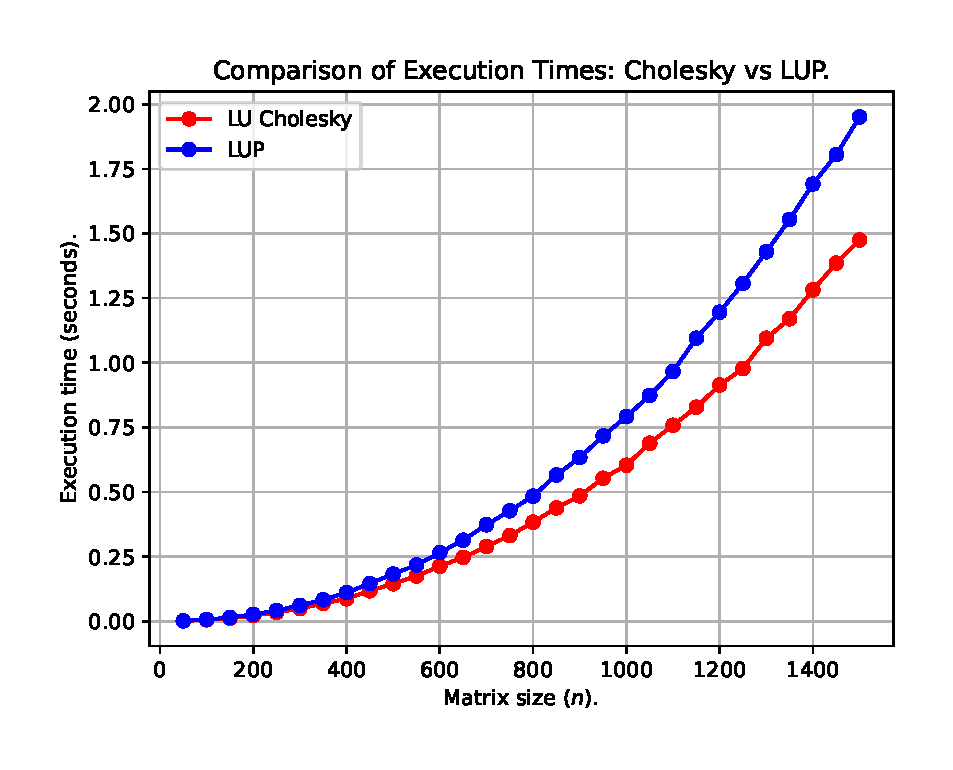
\includegraphics[width=0.74\textwidth]{IMAGENES/Figure_1.pdf}
\end{figure}

Se puede notar que a medida que $n$ crece, el algoritmo LUP se vuelve más costoso que el de la factorización de Cholesky. A pesar de que ambos son de orden $n^{3}$, se puede notar que LUP es menos eficiente.










